\chapter{実装}
%ラズパイマウスのfollowerノードについての実装を書く.今はspheroとラズパイマウスのwiibordを本実装として話しているため改変が必要.aproachに持っていく.
\begin{figure}[ht]
    \centering
    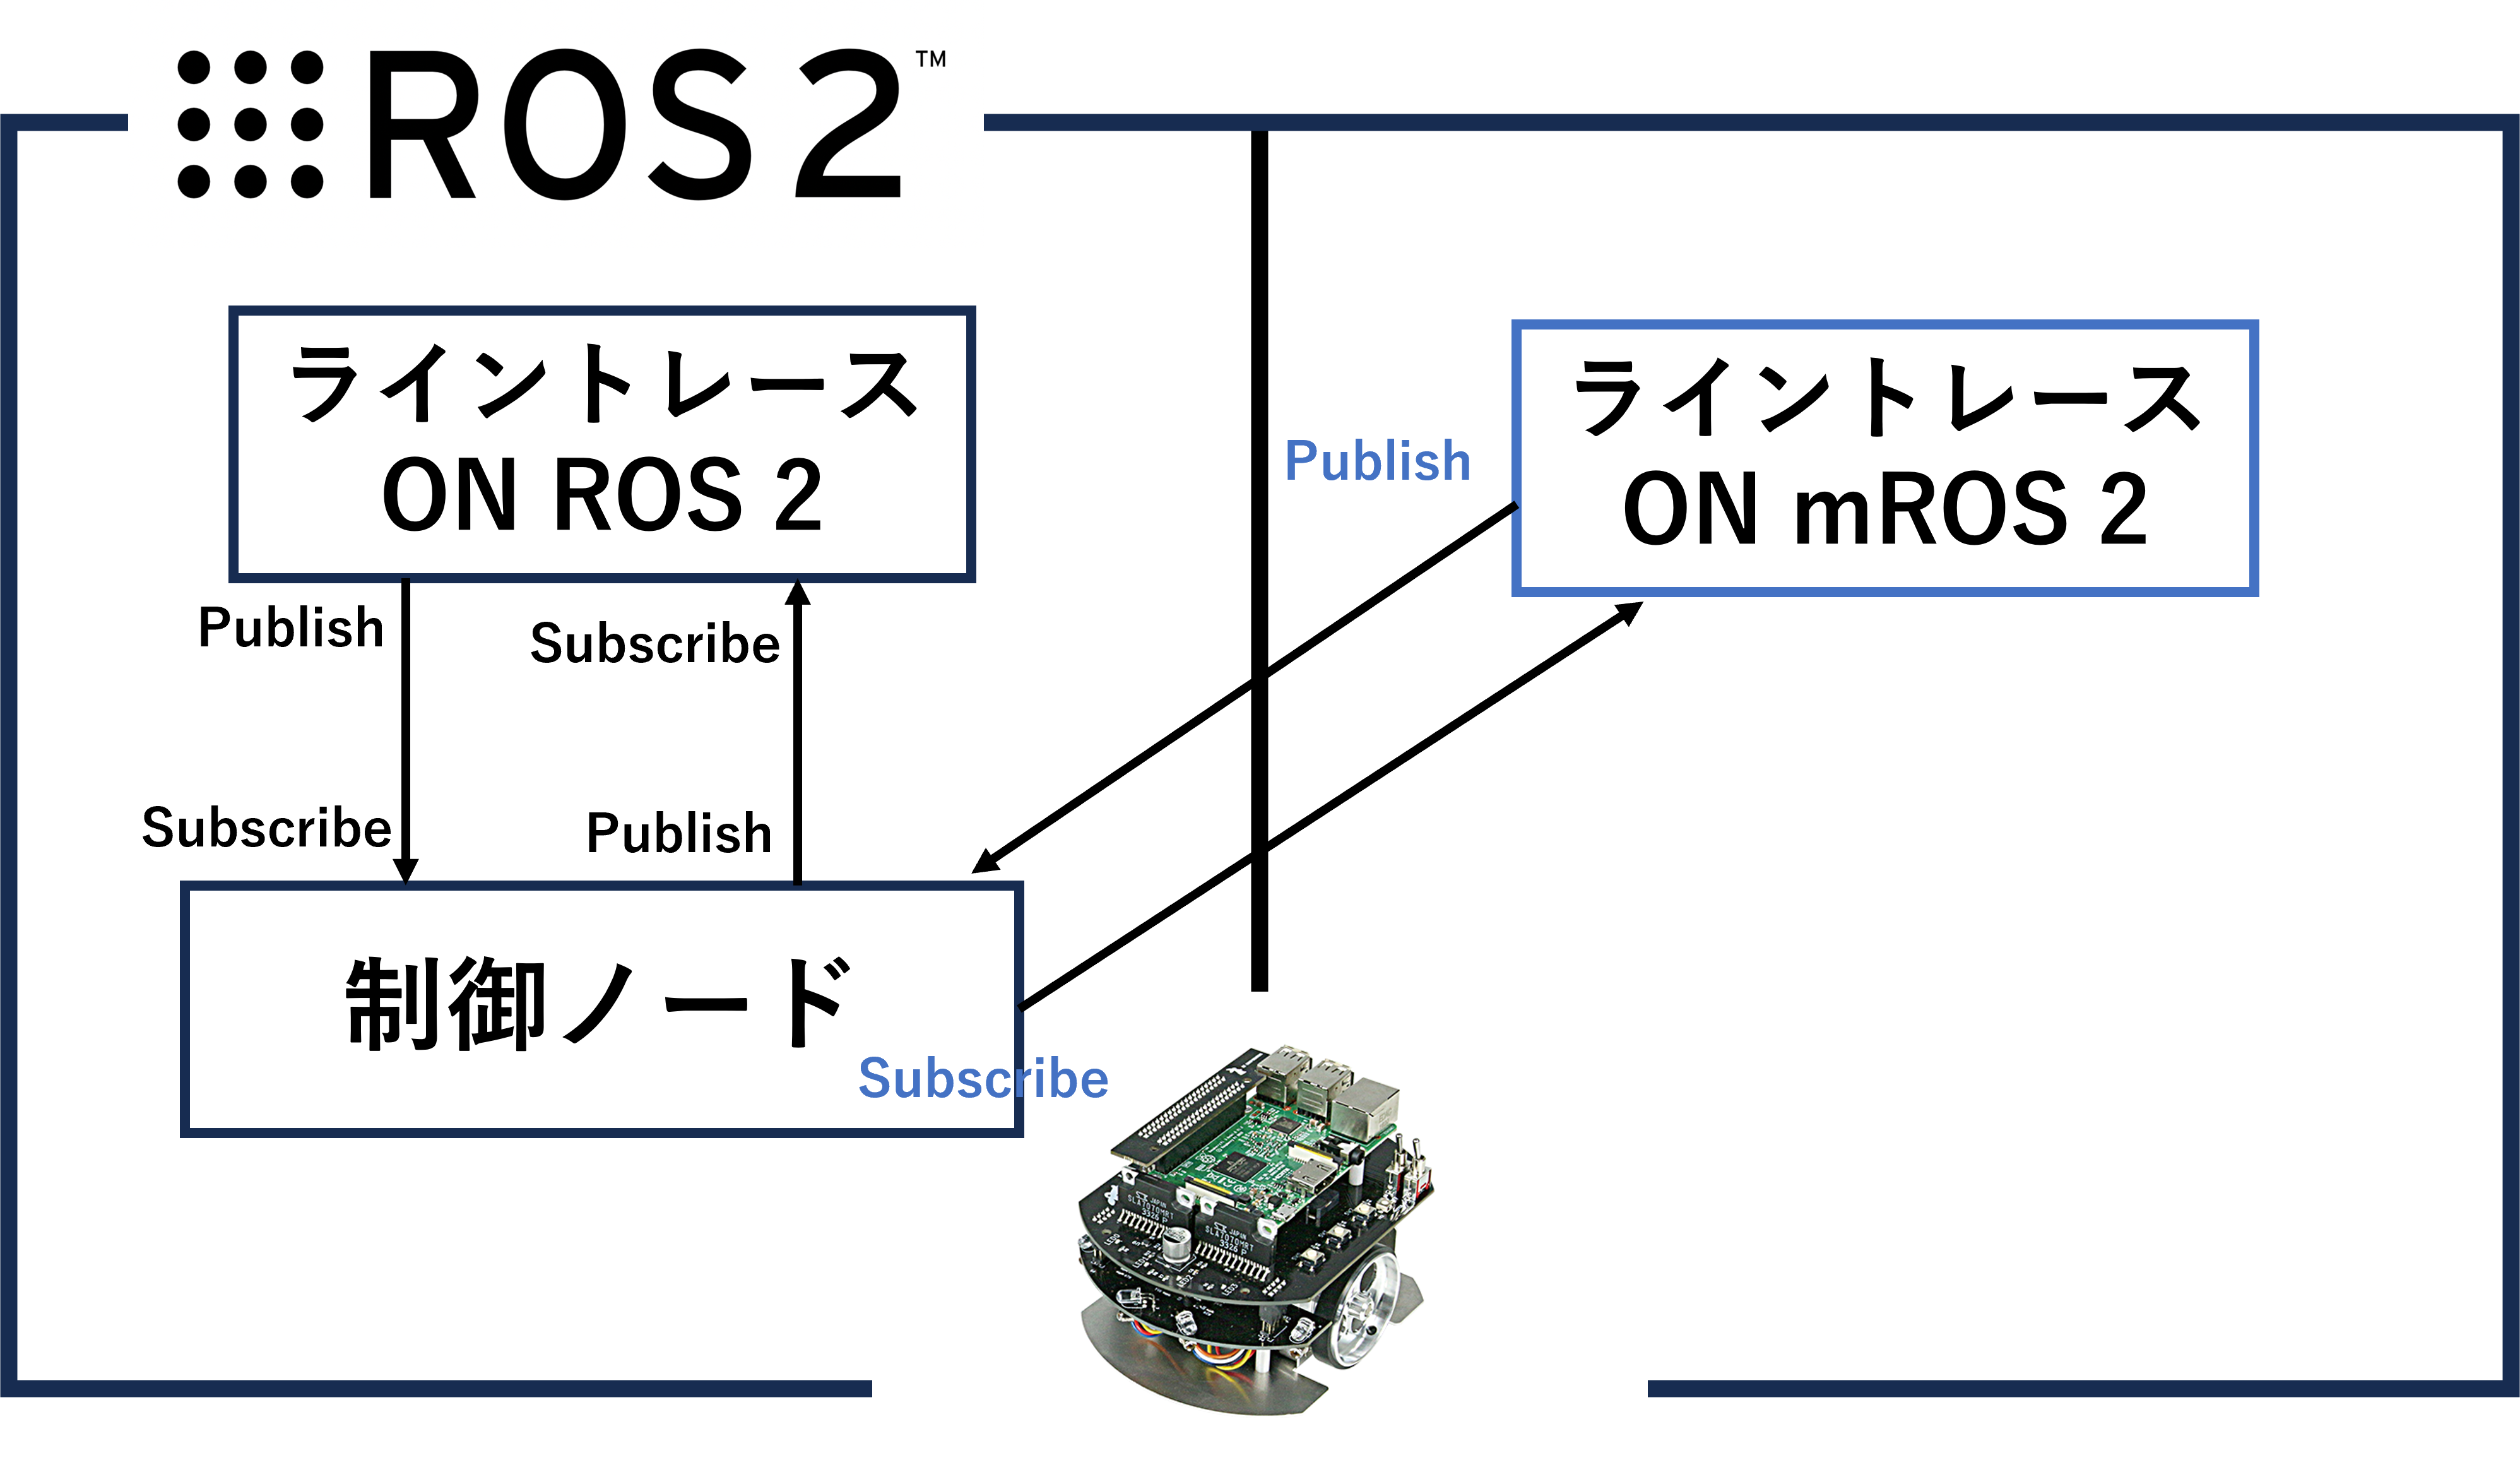
\includegraphics[width=10cm]{images/fig4_raspimouse_configuration.png}
    \caption{実装アプリケーション構成1}
    \label{fig:mros2_ros2_raspimouse_configuration}
\end{figure}
\begin{figure}[h]
    \centering
    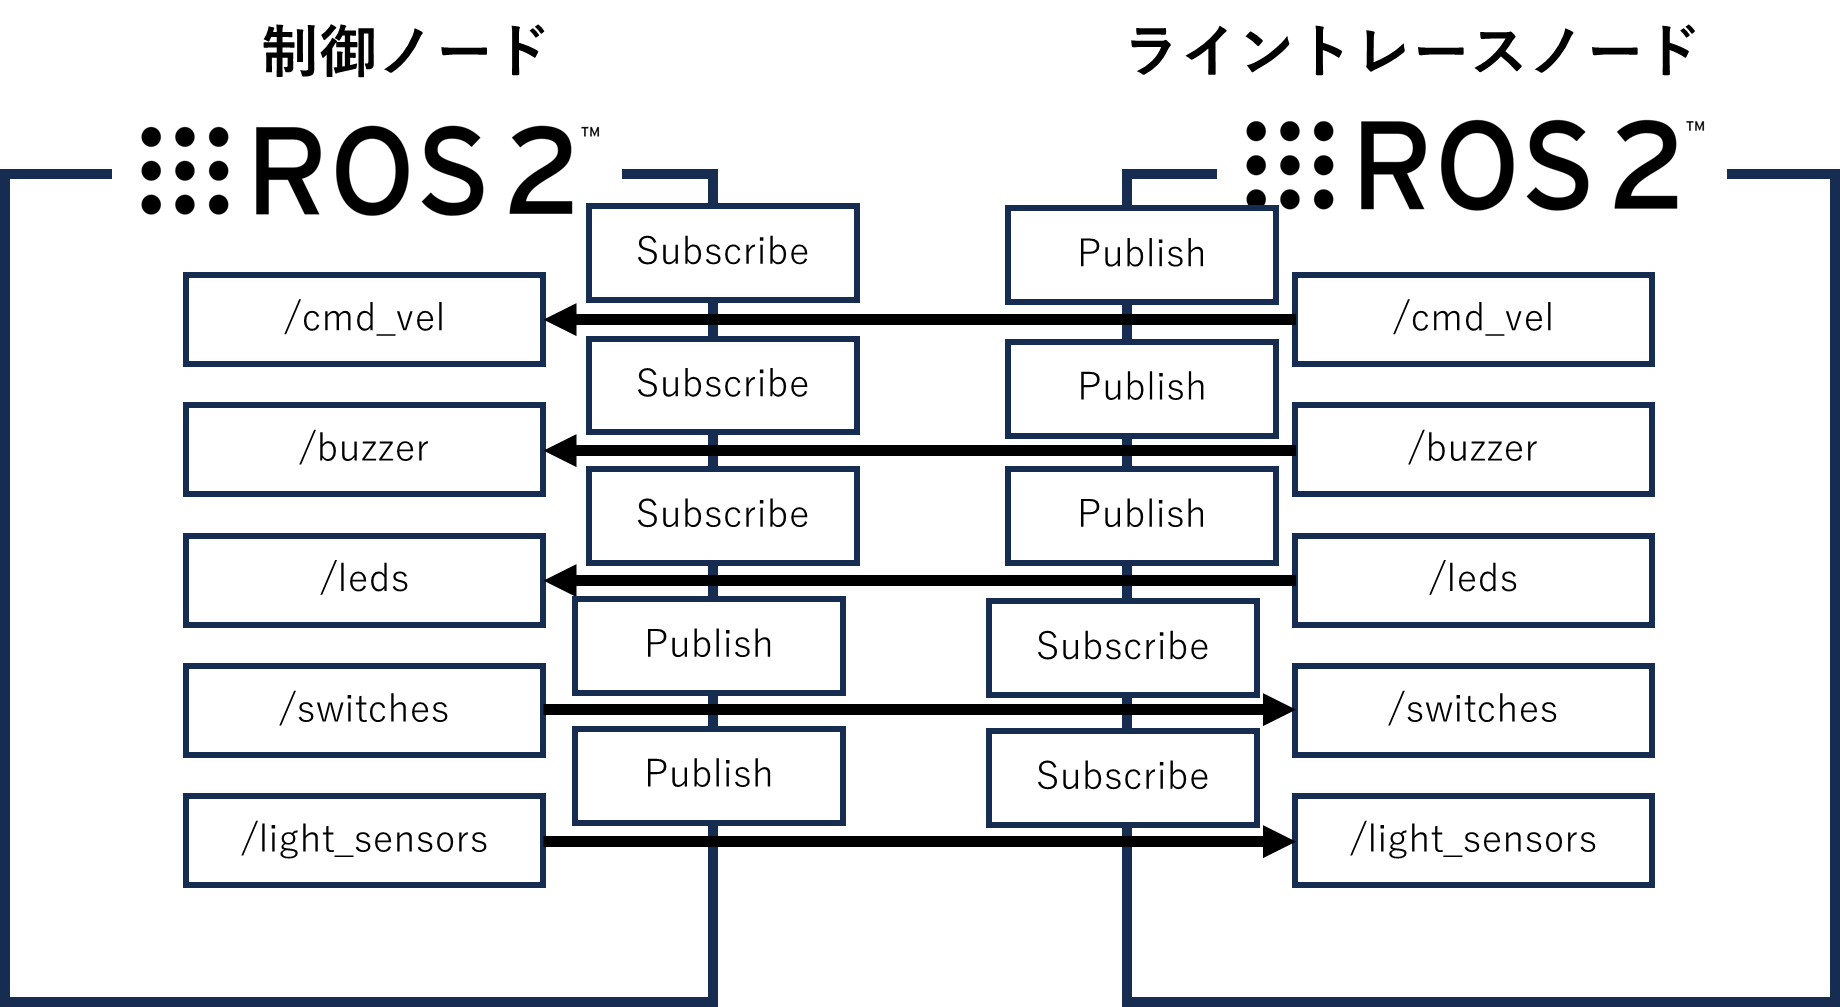
\includegraphics[width=10cm]{images/fig4_pubsub_configuration.png}
    \caption{実装アプリケーションのPub/Sub通信構成}
    \label{fig:mros2_ros2_pubsub_configuration}
\end{figure}
\label{chap:implementation}
%書くこと
%ラズパイマウスのfollowerノードについての実装

本章では,mROS 2-POSIXとROS 2の性能を比較評価するにあたって,mROS 2-POSIXとROS 2に実装するアプリケーションの概要について説明する.
\section{実装アプリケーションの構成}
本研究ではROS 2で動作するライントレースノードをmROS 2-POSIXに移植し,mROS 2-POSIXとmROS 2-wasm,ROS 2の性能を比較評価する.
比較評価のためのアプリケーションの構成図を図4.1,図4.2に示す.
\\ 図4.1はmROS 2-POSIXとmROS 2-wasm,ROS 2の実装アプリケーションの構成である.
図のようにラズパイマウスを制御するノードはosに近い実装になっており,動的配置機構を適用するに適していないと判断した.
したがって,OSに依存しないノードであるライントレースノード(followerノード)をmROS 2-POSIXとmROS 2-wasmそれぞれに実装した.
\\ 図4.2はライントレースノードとその制御ノードのPub/Sub通信についての構成図である.
ライントレースノードと制御ノードは相互に5つのトピックを介して通信を行う.
\begin{itemize}
    \item /light\_sensors
    \item /switches
    \item /cmd\_vel
    \item /buzzer
    \item /leds
\end{itemize}
/light\_sensorsと/switchesはライントレースノードがSubscribeするトピックであり,/cmd\_vel,/buzzer,/ledsはライントレースノードがPublishするトピックである.
/light\_sensorsは制御ノードから常にPublishされるライトセンサの値で,光が反射しやすい白い部分をライトセンサに近づけると取得する整数値が大きくなり,光を吸収する黒に近い部分をライトセンサに近づけると取得できる整数値が小さくなる.
/switchesは/light\_sensors同様に制御ノードから常にPublishされるスイッチの状態を表す値である.
スイッチが押されるとtrueがPublishされ,スイッチが押されていないとfalseがPublishされる.
/cmd\_velはライントレースノードがPublishするトピックであり,ラズパイマウスのモーターを制御するためのトピックである.
/buzzerはライントレースノードがPublishするトピックであり,ラズパイマウスから音を鳴らすことができるトピックである.
/ledsはライントレースノードがPublishするトピックであり,ラズパイマウスのLEDを制御するためのトピックである.
%実装したことを証明したかったらコード追加する???
%これらのトピックを介してPub/Sub通信を行い実際に動作する際のフローを図4.3に示す.
こららのトピックを介してPub/Sub通信を行えるよう,Pythonで記述されたライントレースノードをC++に書き換え,mROS 2-POSIXとmROS 2-wasmに移植した.
また,動作フローなどで通信時間に影響がでないように,ROS 2とmROS 2-POSIX,mROS 2-wasmの動作フローを統一した.
% したがって,図4.3のフローはROS 2とmROS 2-POSIX,mROS 2-wasmの動作フローを示している.
% まず,Switchを介してライトセンサの値を取得する動作を行う.
% プログラム上で保持するライトセンサの値はラインの外側の値と,ラインの内側の値の2つである.
% その後,保持した2つの差を基準にしてラインの外側にいるか内側にいるかを判断し,ラインの外側にいる場合はラインの内側に向かって旋回する動作を行う.

% \section{実装アプリケーションの詳細}
% 本節では,実装アプリケーションの詳細について説明する.
% ROS 2,mROS 2-POSIXで実装するノードはサブスクライブするトピックが2つ,パブリッシュするトピックが3つある.
% サブスクライブするトピックは/light\_sensorsと/switchsである.
% このトピックはラズパイマウス制御ノードが現在のライトセンサの値とスイッチの値をパブリッシュするトピックである.
% light\_sensorsはライトセンサの値はint型で配列になっており,switchsはスイッチの値はbool型で配列になっている.
% それぞれオリジナルのメッセージ型で定義去れており,mROS 2-POSIXではROS 2のメッセージ型を変換するために,mros2\_generator\_msgを用いて生成した.
% これらの値はライントレース制御に使われており,制御ノードからのパブリッシュがあってライントレースは動作する.
% 次に,パブリッシュするトピックは/cmd\_vel,/buzzerおよび/ledsである.
% /cmd\_velはラズパイマウスのモーターを制御するためのトピックであり,/buzzerはラズパイマウスのブザーを制御するためのトピックである.そして,/ledsはラズパイマウスのLEDを制御するためのトピックである.
% /cmd\_velは車輪などによく利用されるgeometory\_msgs/Twistというメッセージ型で定義されている.角速度のangularと線速度のlinearがあり,それぞれx,y,zの値がある.
% /buzzerはInt16型のメッセージ型で定義されており,パブリッシュされた値の大きさでラズパイマウスのブザーの音の大きさが変わる.
% /ledsはraspimouse\_msgs/Ledsというラズパイマウスオリジナルのメッセージ型でパブリッシュされる.boolによって4つあるLEDの点灯,消灯を制御する.
% これらのトピックはライントレース制御ノードがサブスクライブするトピックであり,このトピックを実装ノードによってパブリッシュされることで,ライントレース制御が行われる.
% ROS 2の実装は,既存のライントレースノードを使用した.
% そのため,git cloneコマンドで既存のライントレースノードをダウンロードし,ビルドを行った.
% mROS 2-POSIXの実装は,ROS 2の実装をmROS 2-POSIXに移植した.
% 移植にあたって,パブリッシュやサブスクライブなどのAPIをmROS 2-POSIXのAPIに変更した.
\section{実装アプリケーションの問題と解決策}
\begin{figure}[h]
    \centering
    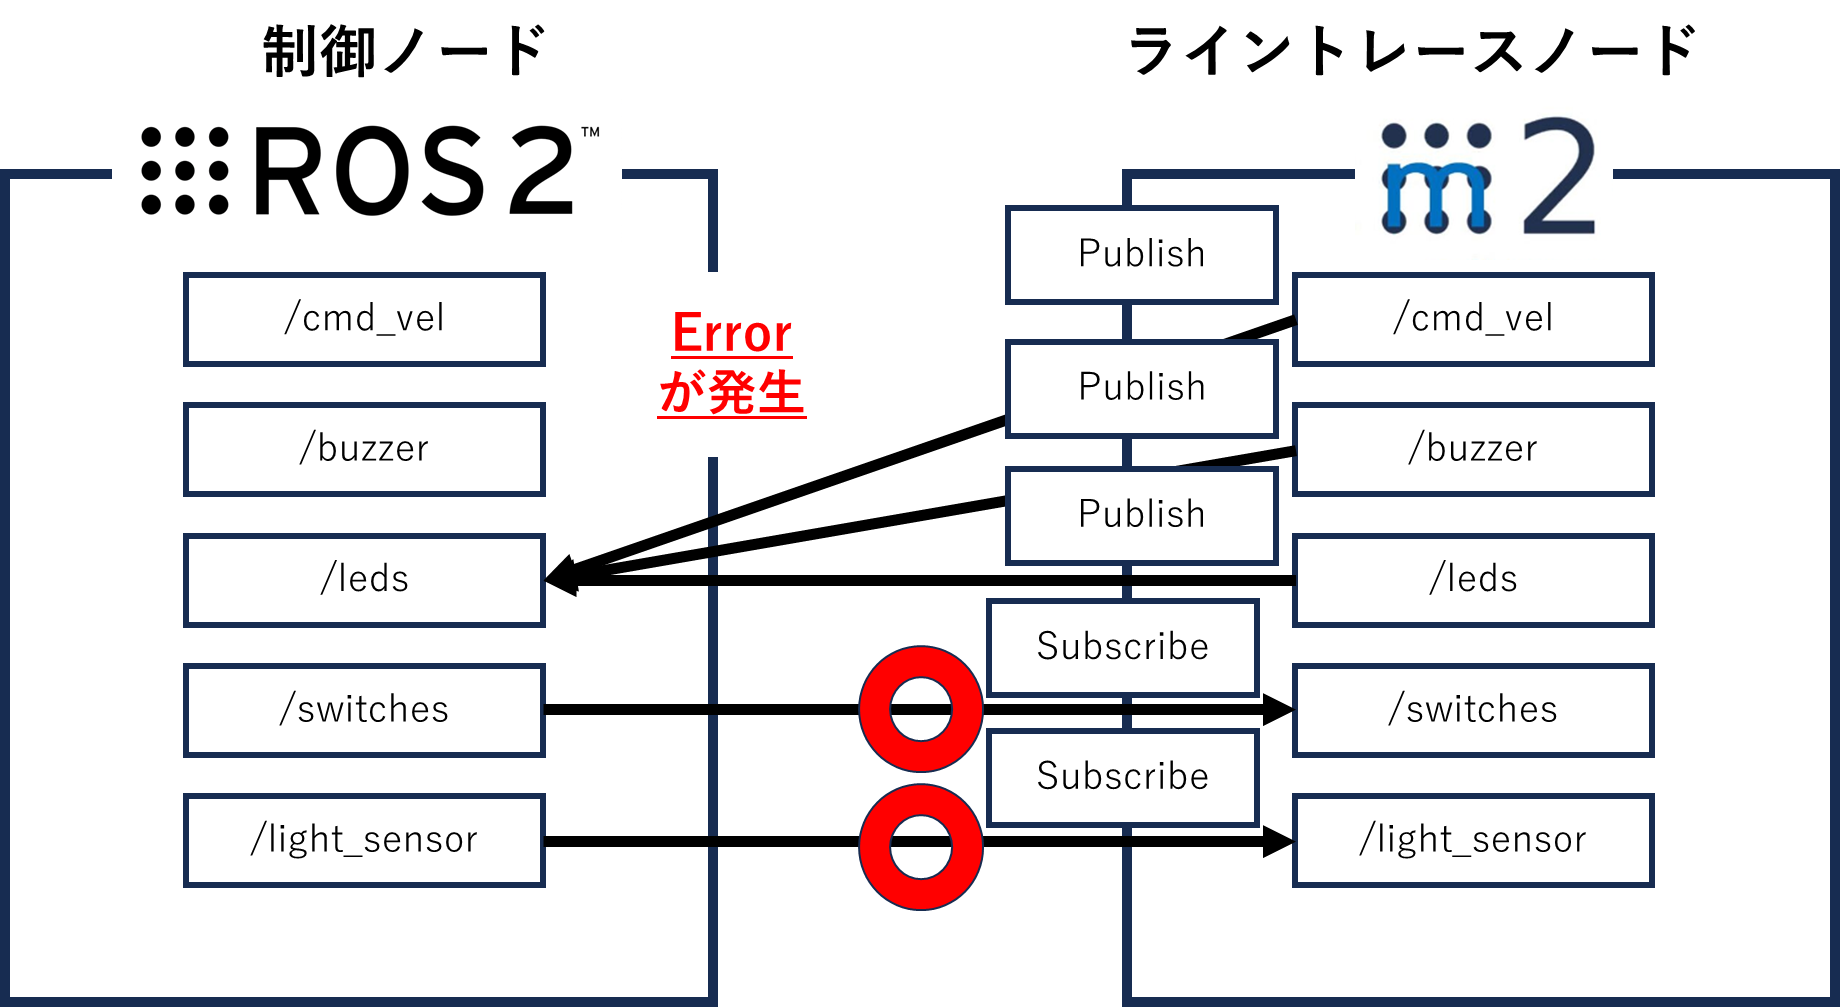
\includegraphics[width=10cm]{images/fig4_mros2bug.png}
    \caption{mROS 2-POSIXのバグ}
    \label{fig:mros2bug}
\end{figure}

\begin{figure}[h]
    \centering
    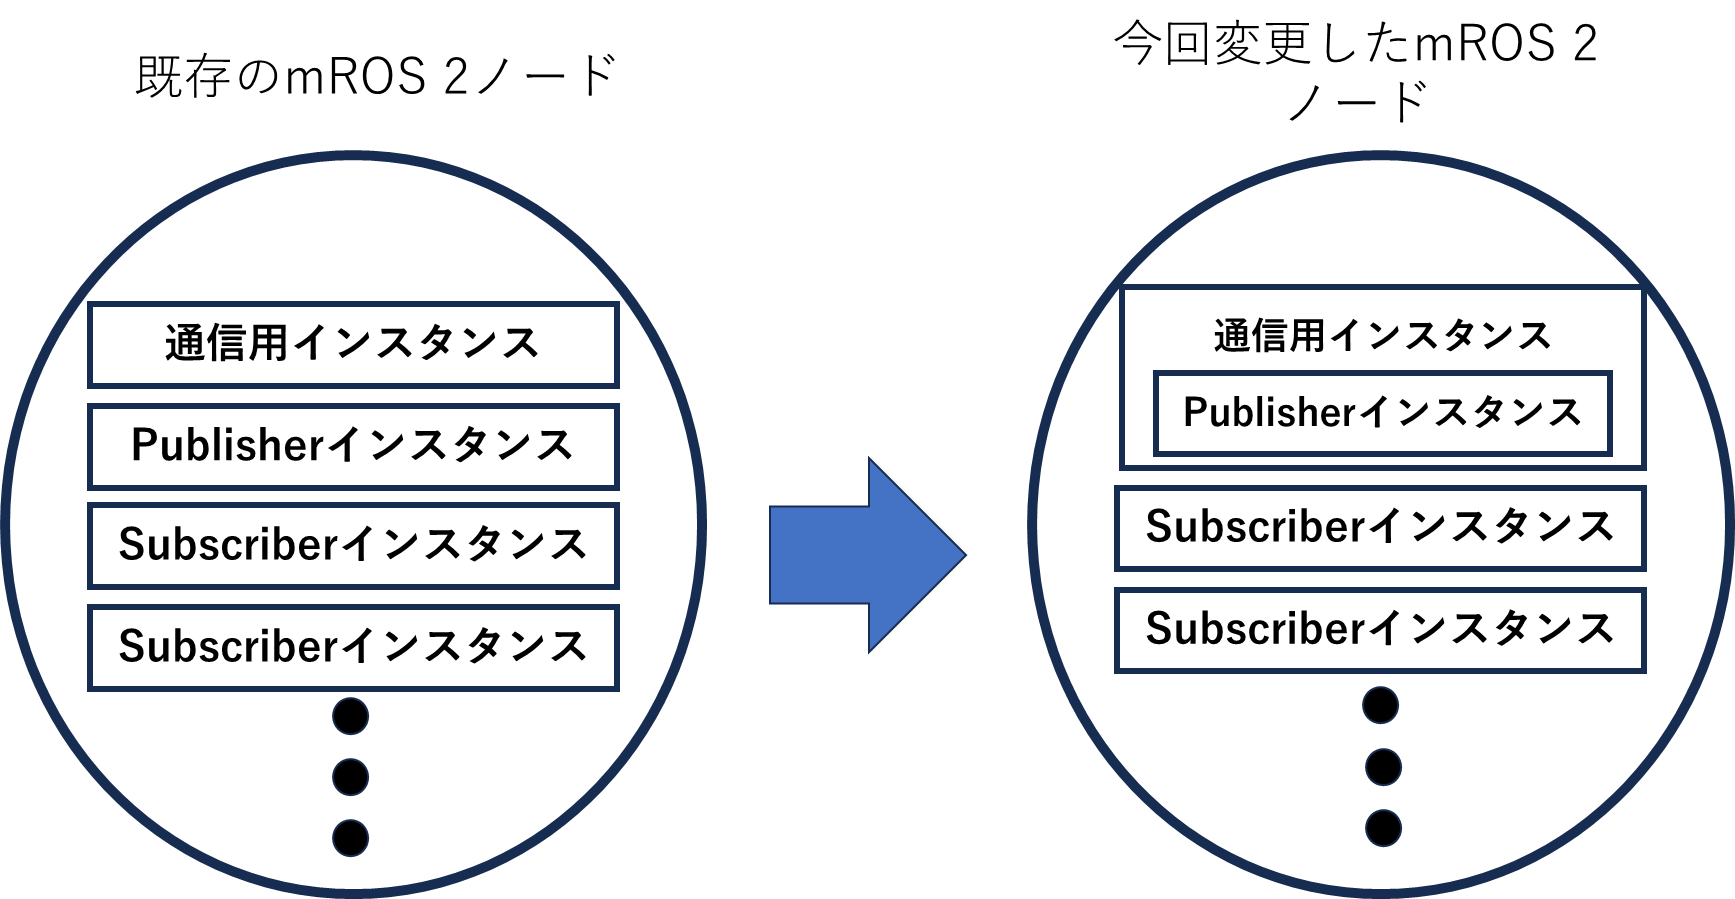
\includegraphics[width=10cm]{images/fig4_mros2bug_fix.png}
    \caption{mROS 2-POSIXのバグ fix}
    \label{fig:mros2bug-fix}
\end{figure}
ROS 2で実装されているノードをmROS 2-posixに実装する際に,mROS 2-posix固有の様々な問題に遭遇した.
以下にその問題を述べる.
\begin{itemize}
    \item mros2-posixのPublisherのバグfix
    \item mros2-posixのQoS設定の変更
    \item mros2-posixのサービス通信が実装されていない
\end{itemize}
%必要性を説いてから問題を書く
%実装課題1:mros2-posixのバグ
%実装課題2:stackしたところはmros2でqosの設定を変更するところ,config
%実装課題3:ラズパイマウスのモーターのon/offにサービス通信を使っているが,mros2-posixにはサービス通信がない
%実装課題4:
mROS 2-POSIXは2024年2月時点で,最後の更新が2年前であり,定期的にメンテナンスされているとは言いにくい.
また,mROS 2-POSIXを評価するにあたって,高瀬らは1つのPublisherとSubscriberを用いたネットワークスループットを評価した.
したがって,実際のアプリケーションのような複数のPublisherとSubscriberを用いるアプリケーションで,mROS 2-POSIX実行しROS 2と通信を試みようとすると,ROS 2のSubscriberでpayloaderrorが発生した.
このerrorはROS 2のSubscriberに対して,想定以上のデータが送信された場合に表示される.
ros2 topic echoを用いてトピックに送信されているデータを確認したところ図4.3に示すように,ROS 2のSubscriberに対してmROS 2-POSIXでPublisherとして定義されているすべてのメッセージが送信されていることが分かった.
これはmROS 2-POSIXのPublisherのインスタンスが1つのみの生成になっていることが原因である.
実装の状態を図4.4に示す.Publisherインスタンスにその情報が上書きされ,最後に作成されたPublisherのトピック宛にすべてのメッセージが送信されている.そのため,本実装では通信用インスタンスに対して,Publisherのインスタンスを生成するように修正した.
\\ mROS 2-POSIXはデフォルトでQoSの設定がBEST\_Effortになっている.
QoSはBest\_EffortとReliableの2つがあり,Best\_Effortはデータの到達を保証しないため,ROS 2ではデフォルトでReliableに設定されている.
PublisherのQoS設定がBest\_Effort,SubscriberのQoS設定がReliableの場合,SubscriberはPublisherからデータを受信できない.
そのため,ROS 2とmROS 2-POSIXのノード間でPub/Sub通信するためには,まず最初にどちらかのQoS設定を変更する必要がある.
mROS 2-POSIXのDDS[]であるembeddedRTPS[]はQoSの設定にReliableとBEST\_Effortをサポートしているため,本実装ではmROS 2-POSIXのQoSをReliableに変更し,対応した.
\\ ROS 2のライントレースノードの実装では,モーターのon/offにサービス通信を使っている.
2章で説明した通り,Service通信はROS 2の通信方法の1つであり,クライアント・サーバーモデルに近い通信方法である.
ROS 2のライントレースノードの実装では,このサービス通信を用いてラズパイマウスのモーターのon/offを操作しているが,mROS 2-posixにはService通信の実装がされておらず,そのまま移植することはできない.
本実装では,mROS 2-POSIXの実装部分でモーターのon/offの処理を削除し,ノードを立ち上げた後,ROS 2の制御ノードに対して端末上からros2 service callを使用することで,モーター電源のon/offを操作した.
これらの問題はmROS 2-Wasmにも同様に存在したが,mROS 2-POSIXを実装する際に解決した方法と同じであったため,省略する.
% ROS 2の実装ではモーター電源のon/offにサービス通信を使っており,mROS 2-POSIXでは第2章で述べた通り,Pub/Sub通信でしか通信することができない.
% そのため,モーターを起動する際は,端末でros2 Service callを使うことでmROS 2-POSIXのパブリッシュからモーターが動作するようにしなければならなった.
% また,第3章のRaspimouseの節で述べたように,ROS 2とmROS 2-POSIXのPub/Sub通信がうまくいかないという問題がある.
% 現在の実装ではそれぞれのパブリッシャー,サブスクライバーのQoS設定をRELIABLEに設定し通信させている.
% ラズパイマウスからのサブスクリプションは常に成功しているが,mROS 2-POSIXからのパブリッシュは部分的に成功している.
% /ledsトピックに対してmROS 2-POSIXからのパブリッシュは成功している.
% しかし,/cmd\_velと/buzzerに対してmROS 2-POSIXからのパブリッシュは失敗していると考えている.
% デバックツールであるros2 topic infoを用いて/cmd\_velと/buzzerのトピックを確認したところ,mROS 2-POSIXからのパブリッシャーは存在しているのにも関わらず,トピックにデータを送信できていなかった.
% これは様々な原因が考えられるが,現在はmROS 2-POSIXの実装に問題があると考えている.
% 理由は,ROS 2制御ノードの端末に [RTPS\_READER\_HISTORY Error] Change payload size of 'X' bytes is larger than the history payload size of '11' bytes and cannot be resized. -> Function can\_change\_be\_added\_nts
% というエラーが出ていることから,mROS 2-POSIXのpayloadが大きすぎるために,パブリッシュが失敗していると考えている.
% この問題を解決するためにためしたことは以下の通りだ.
% \begin{itemize}
%     \item ros2を再構築する
%     \item パブリッシャーとサブスクライバーのQoS設定RELIABLEにする
%     \item 使用するメッセージ型を再生成する
%     \item FastRTPSのHistoryMemoryPolicyをPREALLOCATED\_WITH\_REALLOC\_MEMORY\_MODEに変更する
%     \item FastRTPSのpayload\_max\_size500に変更する
%     \item FastRTPSからCycloneRTPSに変更する
% \end{itemize}
% ros2を再構築したのは,同じエラーに対して,ros2を再構築することでFIXしたという報告があったから試したが,変化はなかった.
% mROS 2-POSIXのパブリッシューとサブスクライバーのQoS設定をRELEABLEにすることで,mROS 2-POSIXのサブスクライバーがパブリッシャーを認識したが,mROS 2-POSIXからのパブリッシュに関して変化はなかった.
% mROS 2-POSIXの更新により,既存のメッセージ型を再構築しないと使えない場合があるので再構築を試したが,変化はなかった.
% payloadの問題に対処するためにFastRTPSの設定を変更するよう.xmlファイルを作り設定したが,設定ファイルを読み込めず,反映できなかった.この原因はわかっていない.
% CycloneRTPSはROS 2のデフォルトのRTPSである.しかしmROS 2-POSIXとの互換性はないようで,CyclonRTPSにした際に,mROS 2-POSIXはROS 2と通信できなくなり,ros2 topic list等のコマンドにも表示されなかった.これはmROS 2-POSIXのRTPSであるembeddedRTPSがCycloneRTPSと互換性がないためだと考えられる.
% 上記の解決策を試したが,いずれも解決には至らなかった.
% 現在,解決方法として考えているのは以下の方法である.
% \begin{itemize}
%     \item mROS 2-POSIXのpayloadの上限を決める
%     \item ROS 2制御ノード側のサブスクリプションのQoS設定のDurabilityをTRANSIENT\_LOCALにする
%     \item rqt consoleやrqt configをPC側から立ち上げ,トピックとデータの流れを確認しながらデバックする
% \end{itemize}


